\documentclass[12pt,a4paper]{article}
% !TEX program = xelatex
\usepackage[utf8]{inputenc}
\usepackage[T1]{fontenc}
\usepackage[finnish]{babel}
\usepackage[utf8]{inputenc}
\usepackage{graphicx}
\usepackage{titling}
\usepackage{titlesec}
\usepackage{booktabs}
\usepackage{fancyhdr}
\usepackage{lipsum}
\usepackage{comment, mdframed}
\usepackage{enumitem}
\usepackage{xcolor}
\usepackage{longtable}
%\usepackage{cite}
\usepackage{pgfgantt}
\usepackage{amsmath, amssymb}
\usepackage{tikz}
\usepackage[margin=1in]{geometry}
\usepackage[backend=biber, style=numeric]{biblatex}
%\usepackage{hyperref}
\usepackage{bookmark}
\usepackage{enumitem}
\usepackage{amsmath}
\usepackage{listings}
\lstset{language=Python, basicstyle=\ttfamily\small, breaklines=true,columns=fullflexible}
\lstset{escapeinside={(*@}{@*)}}
\usepackage{fontspec}
\setmainfont{Arial}
\newfontfamily\stylishfont{Noteworthy}
%\newfontfamily\stylishfont{Zapfino}
%\addbibresource{references.bib}
\usetikzlibrary{calc}
\usepackage{xcolor}

\lstdefinestyle{pidstyle}{
    basicstyle=\ttfamily\footnotesize,
    breaklines=true,
    escapechar=\#, % Define escape character for inline LaTeX commands
    linewidth=\textwidth,
    basicstyle=\ttfamily\scriptsize
}

\renewcommand{\maketitle}{%
  \begin{leftmark}
    \vspace*{\baselineskip} % Add a bit of vertical space

%    \includegraphics[width=4cm]{example-image-a} % Add an image before the title. you will need to replace the image path with your own

%    \vspace{0.5cm} % Add vertical space before title

    \textbf{\fontsize{18}{36}\selectfont \thetitle} % Font Size and Bold Title

     \vspace{0.05cm} % Add vertical space before subtitle
%    \textit{\Large \theauthor}  % Subtitle / Author
    \vspace{\baselineskip} % Add vertical space after subtitle
     \rule{\textwidth}{0.4pt} % Add a horizontal line

   \end{leftmark}
%    \thispagestyle{empty} % Prevent header/footer on the title page
}


% Section Formatting
\titleformat{\section}
  {\normalfont\fontsize{18}{22}\bfseries} % Font and style
  {\thesection}         % Section number
  {1em}                   % Horizontal space after section number
  {}                     % Code before the section name
  []                     % Code after the section name

\titleformat{\subsection}
  {\normalfont\fontsize{14}{18}\bfseries} % Font and style
  {\thesubsection}         % Subsection number
  {1em}                   % Horizontal space after subsection number
  {}                     % Code before the subsection name
  []                     % Code after the subsection name

\setlength{\parindent}{0pt}

\title{Computing platforms (Spring 2025)\newline
week 6}
\author{Juha-Pekka Heikkilä}



\pagestyle{fancy}
\fancyhf{}

\renewcommand{\headrulewidth}{0pt}

\newcommand{\footerline}{\makebox[\textwidth]{\hrulefill}}

\newcommand{\footercontent}{%
    \begin{tabular}{@{}l@{}}
        \footerline \\
        \leftmark \hfill \rlap{\thepage}
    \end{tabular}
}

\fancyfoot[C]{\footercontent}


\newcommand{\exercise}[1]{
    \section*{Tehtävä #1}
    \markboth{Tehtävä #1}{}
}

\addtolength{\hoffset}{-1.75cm}
\addtolength{\textwidth}{3.5cm}
%\addtolength{\voffset}{-3cm}
%\addtolength{\textheight}{6cm}
%\setlength{\parindent}{0pt}



% (a), (b), (c)
\newlist{kohta}{enumerate}{1}
\setlist[kohta,1]{
  label=\textbf{\makebox[1cm][l]{\Huge\text{(\stylishfont\alph*)}}},
  leftmargin=!,
  labelindent=0pt
}

% (1), (2), (3)
\newlist{alakohta}{enumerate}{1}
\setlist[alakohta,1]{
  label=\textbf{\makebox[1cm][l]{\Large\text{(\arabic*)}}},
  leftmargin=!,
  labelindent=0pt
}

% termi: selitys
\newlist{kuvaus}{description}{1}
\setlist[kuvaus]{%
  font=\bfseries\stylishfont,
  labelsep=0.5cm,
  leftmargin=2.5cm,
  style=nextline
}

\newcommand{\korostus}[2][yellow]{\colorbox{#1}{\strut #2}}
%\korostus{Yksi kirjoittaja on jo sisällä}
%\korostus[red]{Lukijan täytyy odottaa jos kirjoittajia on paikalla}
%\korostus[orange]{Tämä osa ei ole suoritettavissa}


\newcommand{\evalslantti}[4][-12]{%
%  \left. #2 \,\right|% ei indeksejä tähän
  \mkern-10mu\raisebox{0pt}[0pt][0pt]{\rotatebox{#1}{$\Big|$}}% vinoviiva päälle
  \mkern3mu{}_{\!#3}^{\!#4}% arvot viivan oikealle puolelle
}


\newcommand{\evalraise}{1.2ex}
\newcommand{\evallow}{1.2ex}

% vino eval-viiva, arvot oikealla (oletus: -12)
% \evalslant[asteet]{lauseke}{ala}{yla}
\newcommand{\evalslant}[4][-12]{%
  \left. #2 \,\right.%
  \mkern-10mu\raisebox{0pt}[0pt][0pt]{\rotatebox{#1}{$\Big|$}}%
  \mkern2mu{}^{\raisebox{\evalraise}{$\scriptstyle #4$}}_{\raisebox{-\evallow}{$\scriptstyle #3$}}%
}



% vino eval-viiva ENNEN lauseketta
% \evalslantpre[asteet]{lauseke}{ala}{yla}
\newcommand{\evalslantpre}[4][-12]{%
  % viiva ja rajat
  \raisebox{0pt}[0pt][0pt]{\rotatebox{#1}{$\Big|$}}%
  \mkern2mu{}^{\raisebox{\evalraise}{$\scriptstyle #4$}}_{\raisebox{-\evallow}{$\scriptstyle #3$}}%
  % itse lauseke
  \mkern4mu\left. #2 \right.%
}


\DeclareMathOperator{\Var}{Var}
\DeclareMathOperator{\Cov}{Cov}
\DeclareMathOperator{\Corr}{Corr}
\usepackage{tikz}
\usetikzlibrary{automata, positioning, arrows}
\usepackage{amssymb,amsmath,graphicx,color}

\newcommand{\set}[1]{\left\{\,#1\,\right\}}
\newcommand{\abs}[1]{\lvert#1\rvert}

\newcommand{\N}{\mathbb{N}}
\newcommand{\Pot}{{\cal P}}

\newcommand{\rma}{\mathrm{a}}
\newcommand{\rmb}{\mathrm{b}}
\newcommand{\rmc}{\mathrm{c}}

\title{TKT20005 Laskennan mallit Viikko3}
\date{}

\begin{document}

\maketitle

\exercise{1 Äärellisen automaatin muodostaminen.} Tässä tehtävässä harjoitellaan muodostamaan äärellinen automaatti annetulle kielelle.
\begin{kohta}
\item
Piirrä deterministinen äärellinen automaatti, joka hyväksyy
tasan ne aakkoston $\set{\mathrm{a},\mathrm{b},\mathrm{c}}$
merkkijonot, jotka päättyvät cba.
\begin{center}
  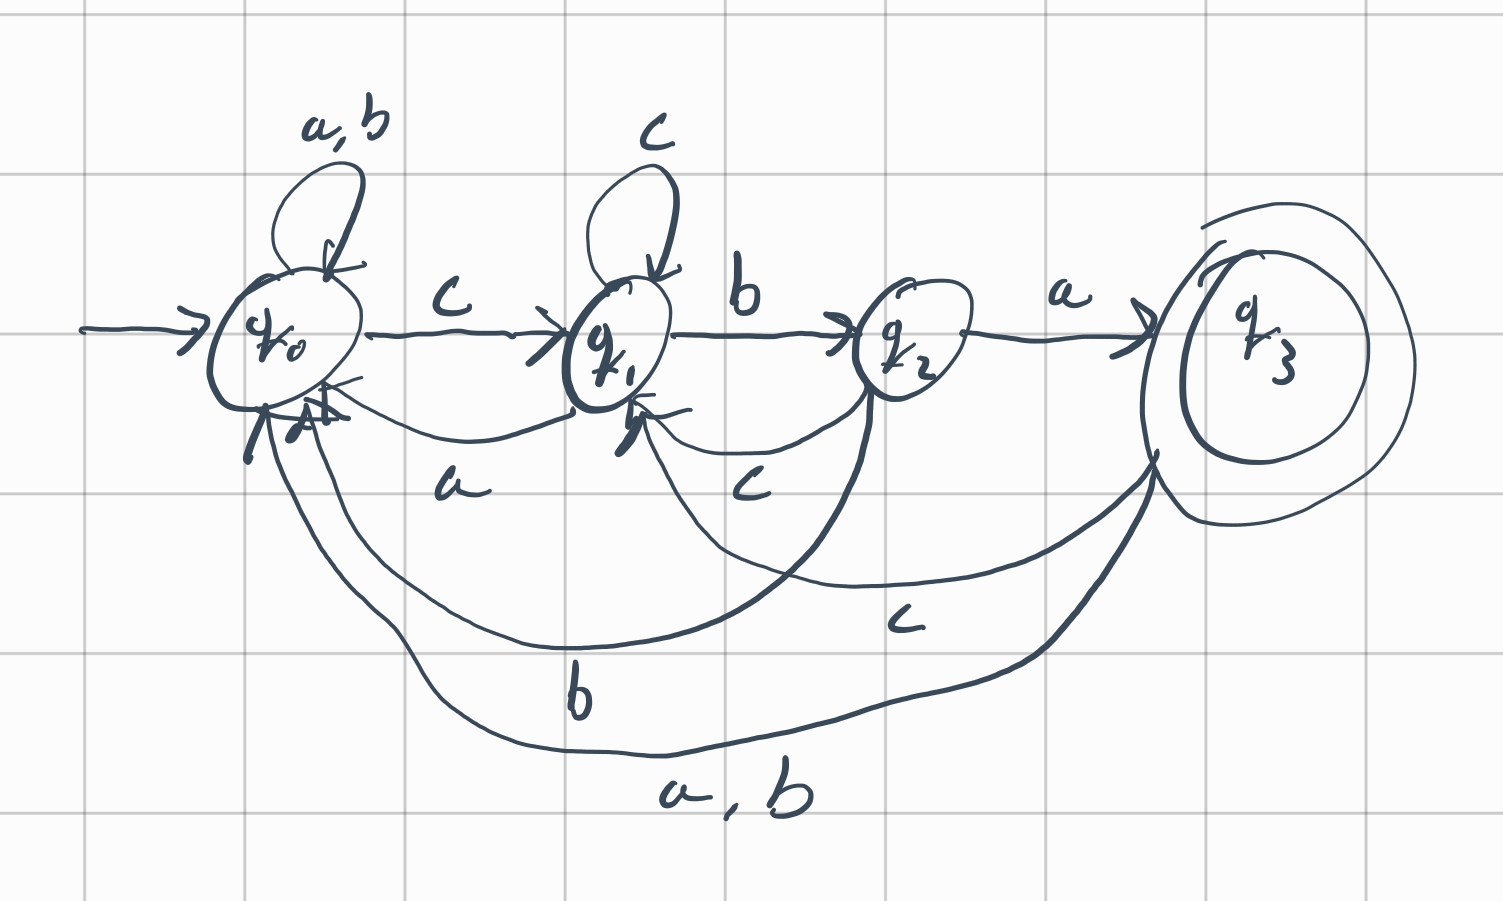
\includegraphics[width=.6\textwidth]{viikko3tehtävä1a.jpg}
\end{center}

\item
Piirrä deterministinen äärellinen automaatti, joka hyväksyy tasan ne 
aakkoston $\set{\mathrm{a},\mathrm{b},\mathrm{c}}$ merkkijonot,
jotka eivät sisällä osamerkkijonoa bc.\\
\begin{center}
  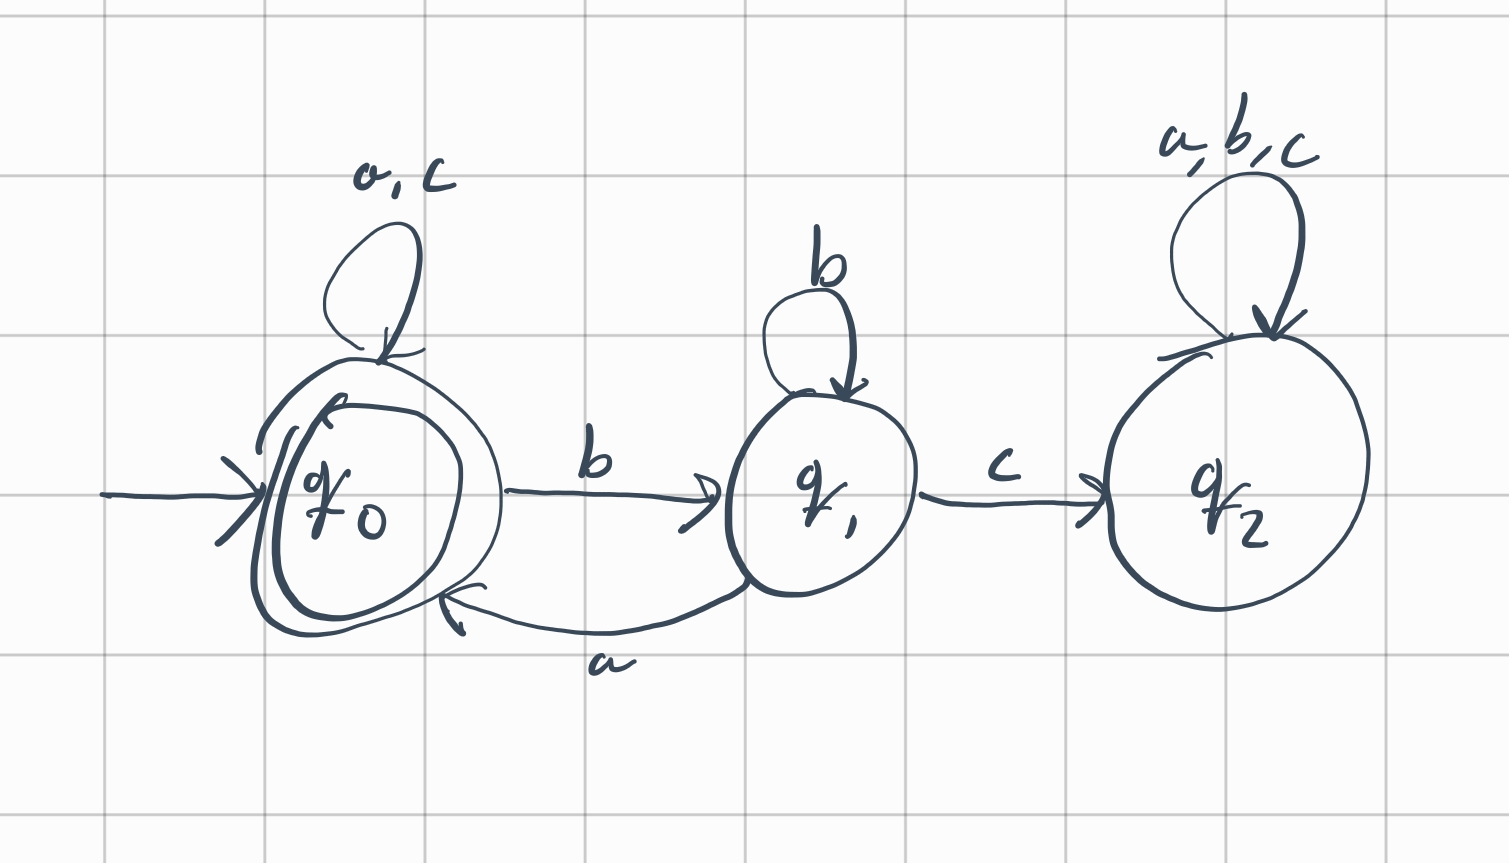
\includegraphics[width=.6\textwidth]{viikko3tehtävä1b.jpg}
\end{center}

\item
Piirrä deterministinen äärellinen automaatti, joka hyväksyy tasan ne 
aakkoston $\set{\mathrm{a},\mathrm{b},\mathrm{c}}$ merkkijonot,
joissa jokainen paritonnumeroinen merkki on b.
\begin{center}
  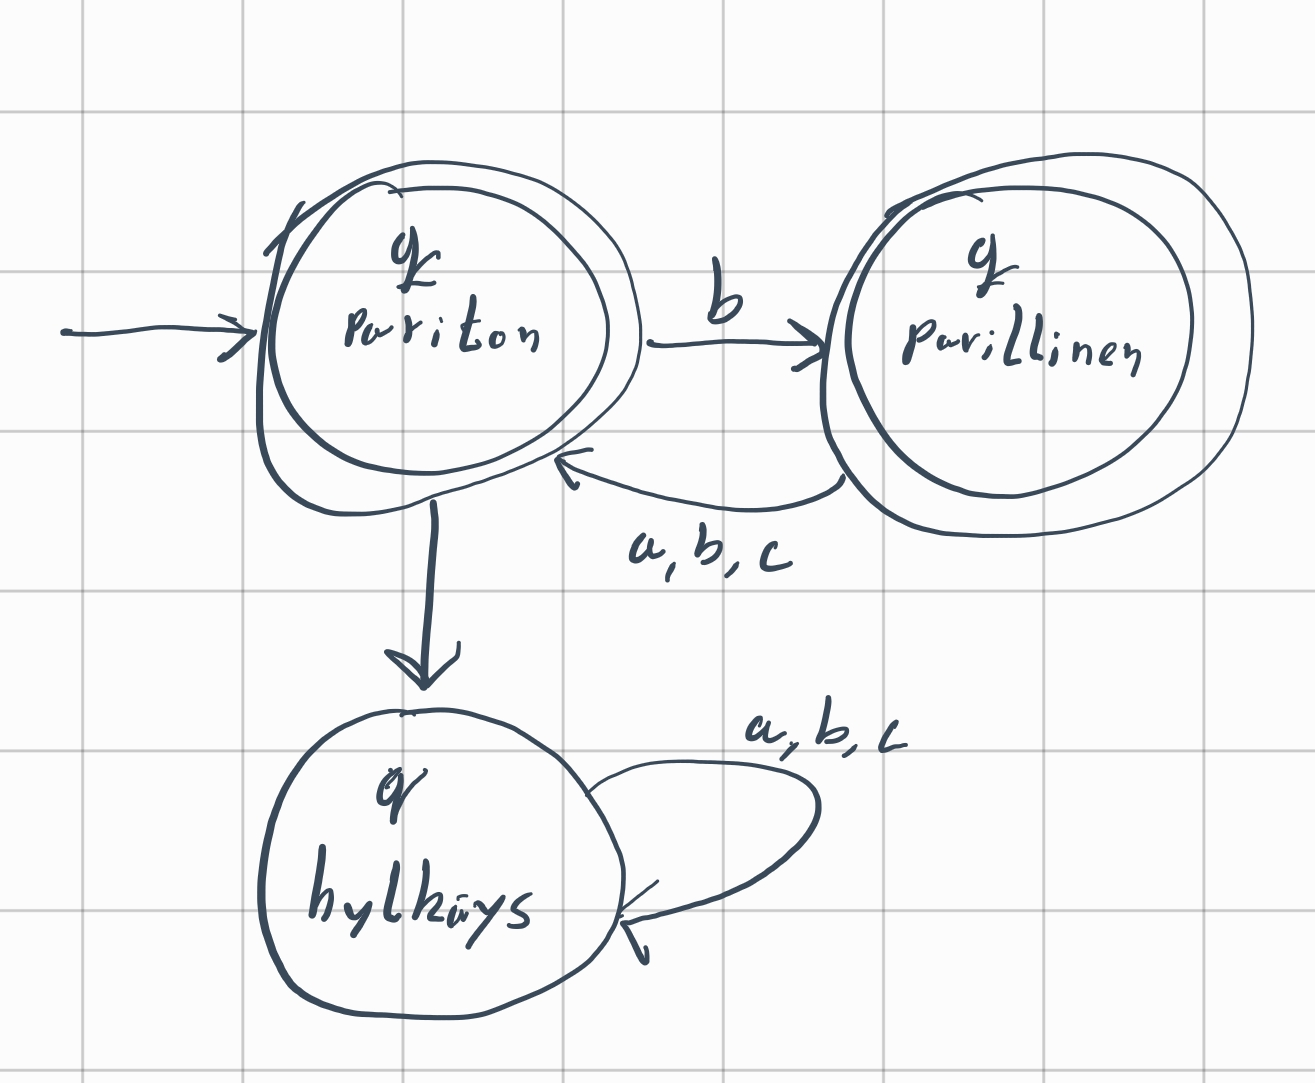
\includegraphics[width=.6\textwidth]{viikko3tehtävä1c.jpg}
\end{center}
Automaatti seuraa ollaanko lukemassa paritonta vai parillista merkkiä jonossa.

\item
Piirrä deterministinen äärellinen automaatti, joka hyväksyy tasan ne 
aakkoston $\set{\mathrm{a},\mathrm{b},\mathrm{c}}$ merkkijonot,
joissa a- ja b-merkkien lukumäärien erotus on
pariton.
\begin{center}
  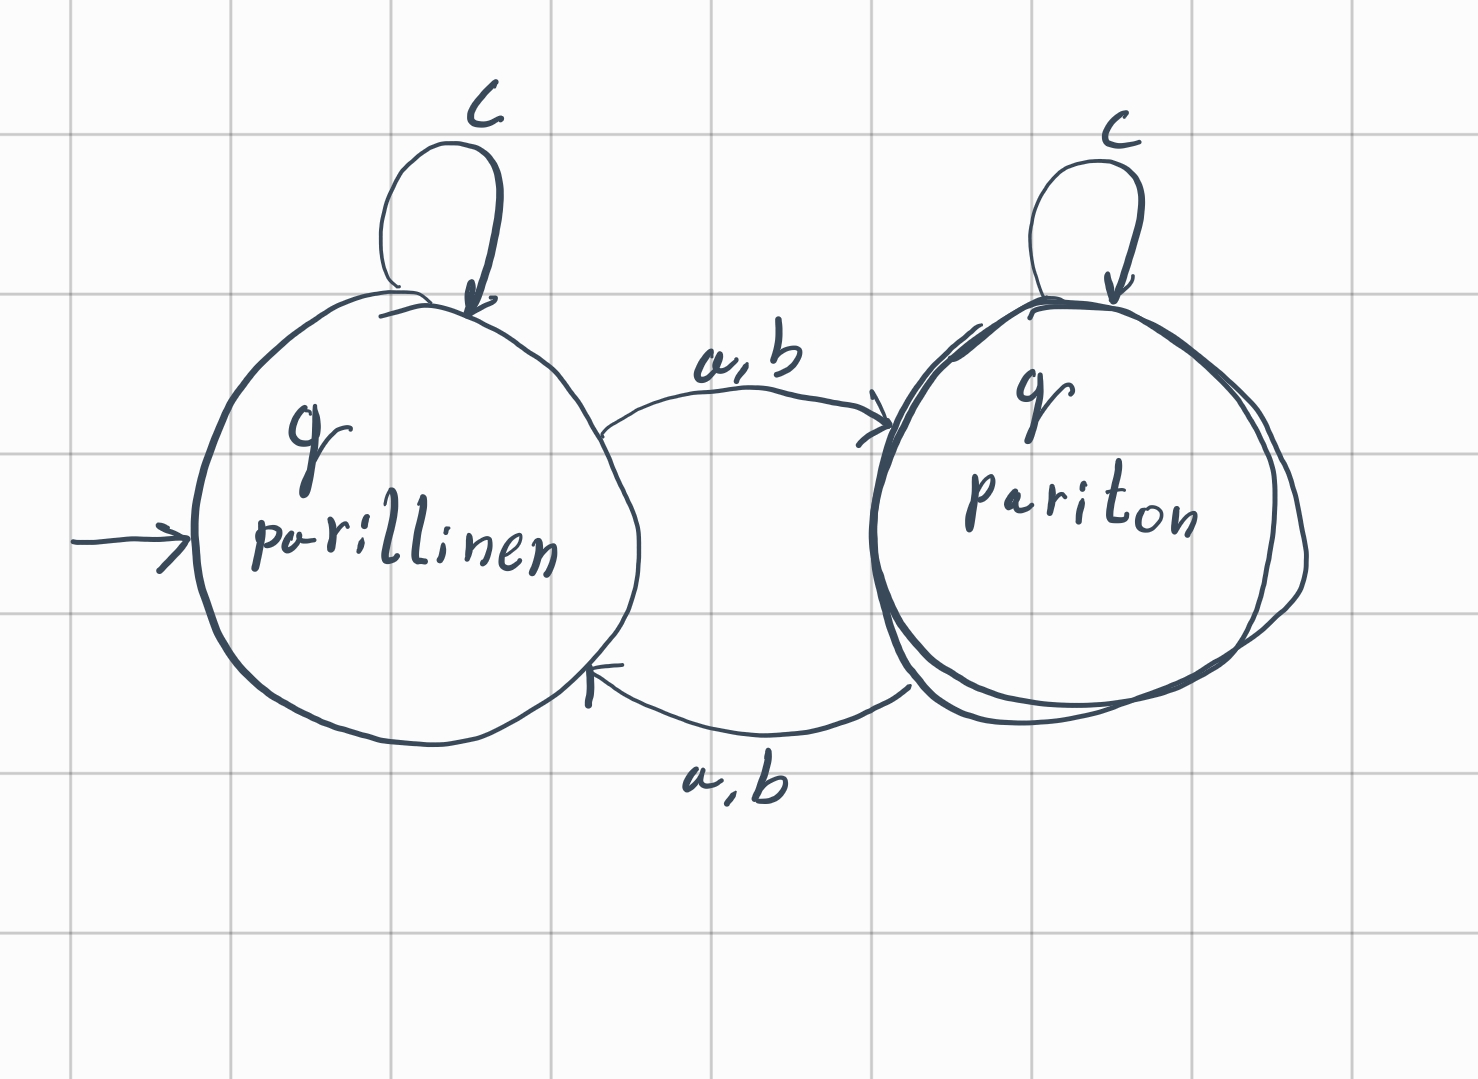
\includegraphics[width=.6\textwidth]{viikko3tehtävä1d.jpg}
\end{center}
'c' lukumäärä ei vaikuta. $|N_a - N_b|$ on pariton jos summa $N_a + N_b$
on pariton. Voidaan siis seurata a- ja b-merkkien yhteismäärän pariteettia.

\end{kohta}








\pagebreak
\exercise{2. Muunnos epädeterministisestä automaatista deterministiseksi.}

\begin{alakohta}
\item \textbf{NFA $\to$ DFA}

DFA alku on $\{1\}$. Hyväksyviä ovat osajoukot missä on $4$

\medskip
\noindent Siirtymätaulukko:
\[
\begin{array}{c|cc}
\text{\sigma} & a & b \\\hline
\{1\}   & \{2,4\} & \{2,4\} \\
\{2,4\} & \varnothing & \{1,3\} \\
\{1,3\} & \{2,4\} & \{2,4\} \\
\varnothing & \varnothing & \varnothing
\end{array}
\]


Hyväksyvä: $\{2,4\}$. Alkutila: $\{1\}$.

\begin{center}
  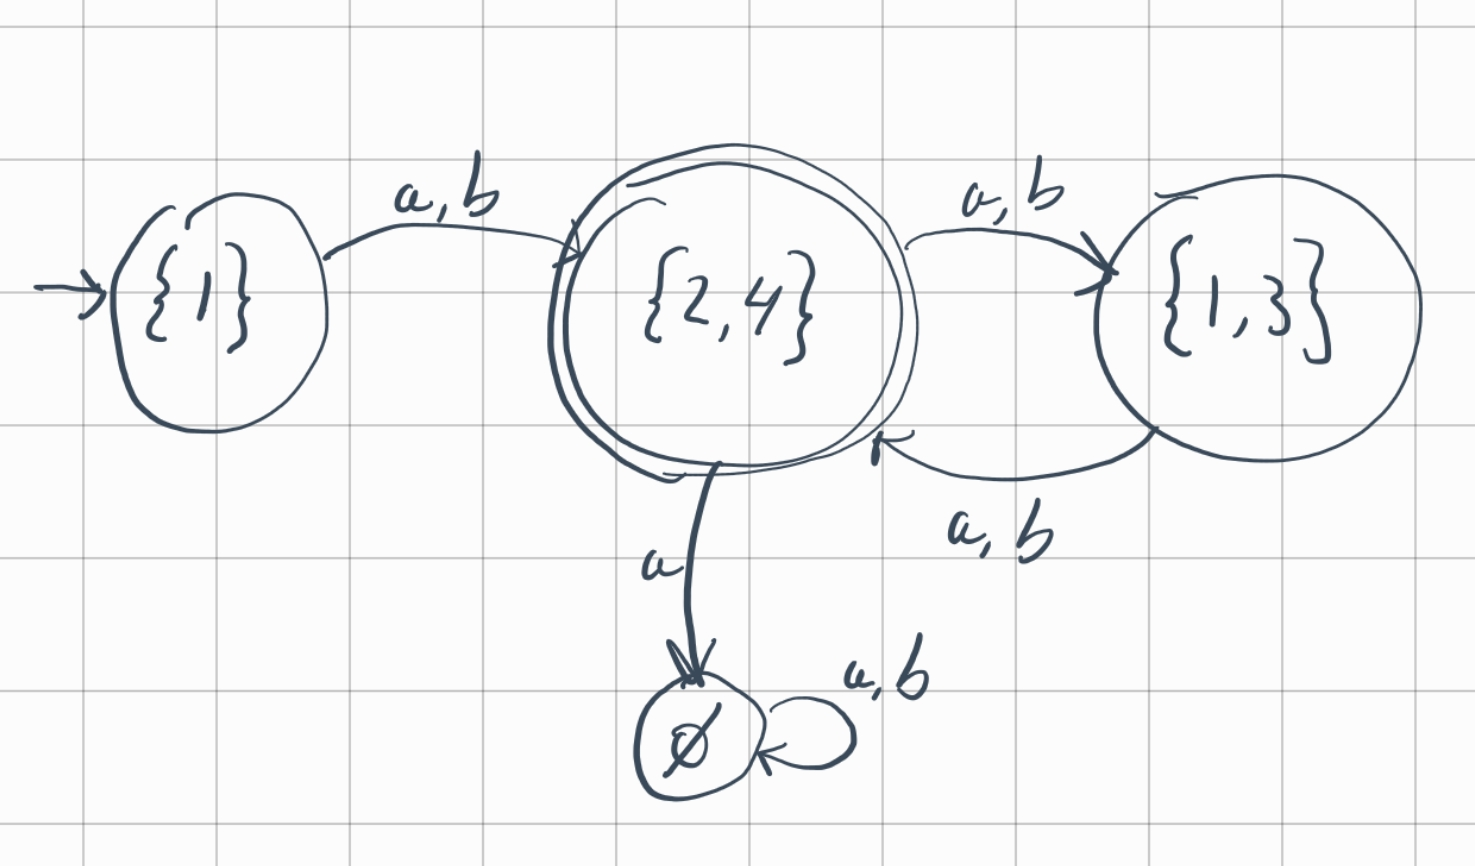
\includegraphics[width=.5\textwidth]{viikko3tehtävä21.jpg}
\end{center}


\item \textbf{Voiko DFA:ta yksinkertaistaa?} \\
Kyllä. \{1\} ja \{1,3\} kummastakin a ja b vievät aina samaan
tilaan \{2,4\}, ja kumpikaan ei ole hyväksyvä
jolloin ne voidaan yhdistää.

\medskip
\noindent Minimoitu siirtymätaulukko
\[
\begin{array}{c|cc}
\text{\sigma} & a & b \\\hline
S\ (\{1\}\!=\!\{1,3\}) & T & T \\
T\ (\{2,4\}) & D & S \\
D\ (\varnothing) & D & D
\end{array}
\]
Alku S (ei-hyväksyvä), hyväksyvä T, D on ikiluuppi.

\begin{center}
  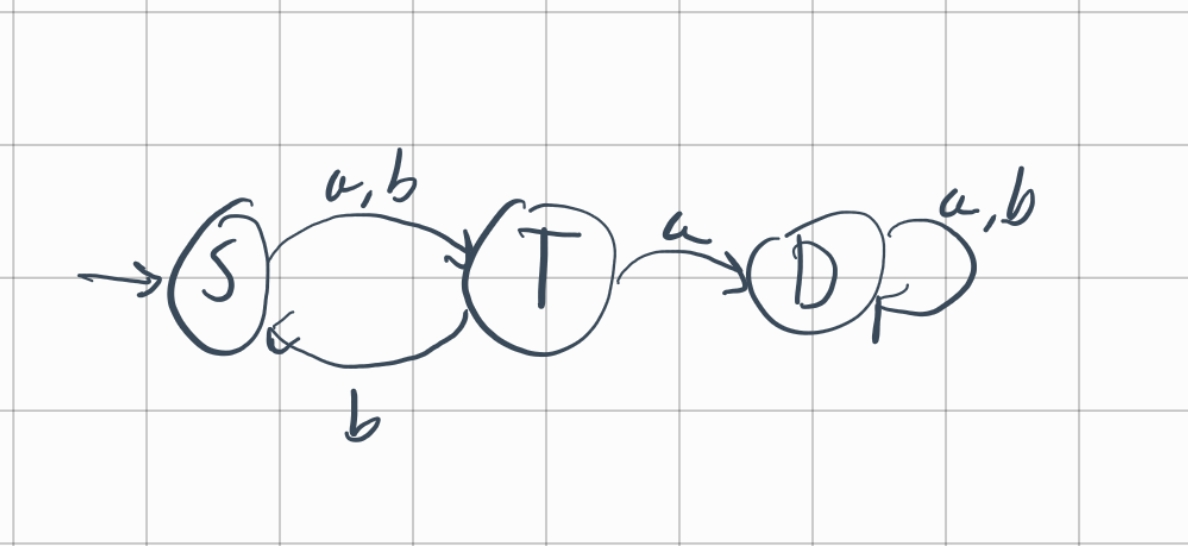
\includegraphics[width=.5\textwidth]{viikko3tehtävä22.jpg}
\end{center}

\end{alakohta}






\pagebreak
\exercise{3. Säännöllisten kielten sulkeumat.}

Mitkä seuraavista väitteistä pitävät paikkansa?
Perustele vastauksesi todistamalla väite tai antamalla vastaesimerkki.
Perusteluissa voit pitää tunnettuina kurssilla tähän asti
esitetyt tulokset sekä sen, että esim.\ kieli $C=\set{0^n1^n\mid n\in\N}$
ei ole säännöllinen.
\begin{kohta}
\item
Jos $A$ on säännöllinen ja $B$ on säännöllinen, niin
$A\cup B$ on säännöllinen.\\

Pitää painkansa. \\
Jos $A$ ja $B$ ovat säännöllisiä, on olemassa DFA:t $M_A$ ja $M_B$.
Automaatti M tiloilla $Q_A\times Q_B$ tunnistaa $A\cup B$ (hyväksyvät tilat
$\{(p,q)\mid p\in F_A \text{ tai } q\in F_B\}$). Siis $A\cup B$ on säännöllinen

\item %b
Jos $A$ on säännöllinen ja $B$ ei ole säännöllinen, niin
$A\cup B$ ei ole säännöllinen.\\

Ei pidä paikkaansa.\\
Vastaesimerkki: Olkoon $A=\Sigma^{\*}$ (säännöllinen, niin iso
että $B\subseteq A$) ja $B=\{0^n1^n\mid n\in\mathbb{N}\}$
(ei säännöllinen). Tällöin $A\cup B=\Sigma^{\*}$ on säännöllinen.\\
\item %c
Jos $A$ on säännöllinen ja $A\cup B$ ei ole säännöllinen,
niin $B$ ei ole säännöllinen.\\

Pitää paikkansa.\\
Jos $A$ on säännöllinen ja $A\cup B$ ei ole säännöllinen,
niin $B$ ei voi olla säännöllinen.\\

\item %d
Jos $A$ ei ole säännöllinen ja $B$ ei ole säännöllinen,
niin $A\cap B$ ei ole säännöllinen.\\

Ei pidä paikkaansa.\\
Kaksi ei-säännöllistä voivat leikata säännölliseksi.
Vastaesimerkki:
\[
A=\{0^n1^n\mid n\ge 0\},\qquad
B=\{0^n1^{n+1}\mid n\ge 0\} \quad\mid \text{kummassakaan ei yhtään samaa sanaa}
\]
Molemmat ovat ei-säännöllisiä, mutta
$A\cap B=\varnothing$ on säännöllinen.\\
\item
Jos $A$ on säännöllinen ja $B\subseteq A$, niin $B$ on
säännöllinen.\\

Ei pidä paikkaansa.\\
Säännöllisen joukon alajoukko voi olla ei-säännöllinen.
Vastaesimerkki: $A=\Sigma^{\*}$ on säännöllinen ja
$B=\{0^n1^n\}\subseteq A$ ei ole säännöllinen

\item
Jos $B$ on säännöllinen ja $B\subseteq A$, niin $A$ on
säännöllinen.\\

Ei pidä paikkaansa\\
Säännöllinen joukko ei pakota yläjoukkoa säännölliseksi.
Vastaesimerkki: $B=\varnothing$ (säännöllinen) ja
$A=\{0^n1^n\}$ (ei säännöllinen), jolloin
$B\subseteq A$ mutta $A$ ei ole säännöllinen
\end{kohta}







\pagebreak
\exercise{4. Yhdisteautomaatti.} Tämä tehtävä auttaa ymmärtämään luennoilla esitetyn yhdisteautomaatin konstruktion käymällä läpi yhden esimerkin yhdisteautomaatista.
  
Muodosta alla annettuista kahdesta äärellisestä automaatista
deterministinen yhdisteautomaatti luennolla esitetyllä menetelmällä.
Esitä yhdisteautomaatin laskenta syötteellä 0110.
\begin{center}
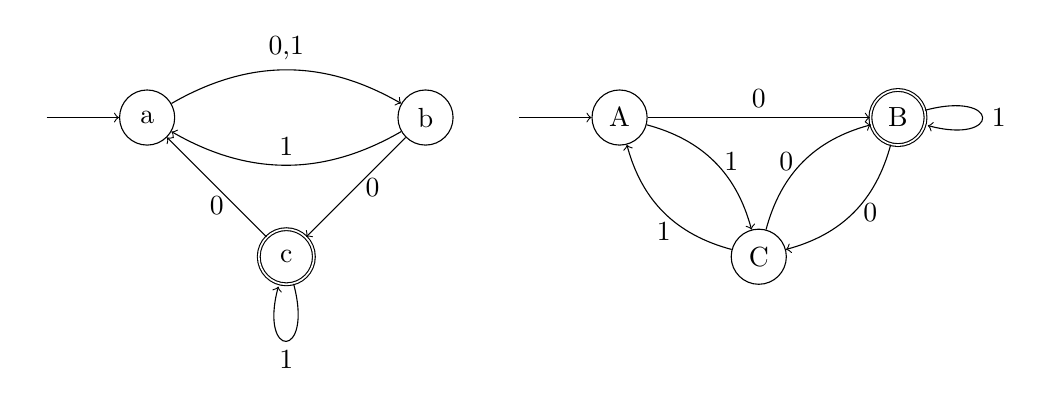
\begin{tikzpicture}[node distance=2.5cm, scale=2.0]
\tikzstyle{state}=[circle,fill=none,draw,minimum size=0.7cm]
\node (start) at (-0.7,0) {};
\node[state] (a) at (0,0) {a};
\node[state,double] (c) [below right of =a] {c};
\node[state] (b) [above right of =c] {b};
\path[-{>[]}]
(start) edge (a)
(a) edge [bend left = 30] node [above] {0,1} (b)
(b) edge node [right] {0} (c)
(b) edge [bend left = 30] node [above] {1} (a)
(c) edge node [below] {0} (a)
(c) edge [loop below] node [below] {1} (c)
;
\tikzstyle{state}=[circle,fill=none,draw,minimum size=0.7cm]
\node (start) at (2.3,0) {};
\node[state] (A) at (3,0) {A};
\node[state] (C) [below right of =A] {C};
\node[state,double] (B) [above right of =C] {B};
\path[-{>[]}]
(start) edge (A)
(A) edge node [above] {0} (B)
(A) edge [bend left = 30] node [right] {1} (C)
(B) edge [bend left = 30] node [right] {0} (C)
(B) edge [loop right] node [right] {1} (B)
(C) edge [bend left = 30] node [left] {0} (B)
(C) edge [bend left = 30] node [below] {1} (A)
;
\end{tikzpicture}
\end{center}
\medskip
Tehdään yhdisteautomaatti. (LaMa luentomateriaali s.54 alkavaan esimerkkiä mukaillen)\\

Vasemman automaatin tilat
$\{a,b,c\}$ (alku $a$, hyväksyvä $c$) ja oikean 
$\{A,B,C\}$ (alku $A$, hyväksyvä $B$)\\

DFA:
\[
M=(Q,\Sigma,\delta,(a,A),F)\qquad
Q=\{a,b,c\}\times\{A,B,C\}\ \ \Sigma=\{0,1\}
\]
\[
\delta\big((p,q),x\big)=(\delta_1(p,x),\delta_2(q,x))\qquad
F=\big(\{c\}\times\{A,B,C\}\big)\ \cup\ \big(\{a,b,c\}\times\{B\}\big)
\]
Eli $(p,q)$ on hyväksyvä, jos jompikumpi komponenteista olisi hyväksyvä
alkuperäisessä automaatissa.
(s.60 LaMa "Tila on hyväksyvä, jos se vastaa ainakin toisen
alkuperäisen automaatin hyväksyvää tilaa")

\bigskip
Saavutettavat tilat ja siirtymät (keltainen = hyväksyvä):

\[
\renewcommand{\arraystretch}{1.15}
\begin{array}{c|cc}
\text{tila} & 0 & 1\\\hline
(a,A)            & \korostus{(b,B)} & (b,C) \\
\korostus{(b,B)} & \korostus{(c,C)} & \korostus{(a,B)} \\
(b,C)            & \korostus{(c,B)} & (a,A) \\
\korostus{(a,B)} & (b,C)            & \korostus{(b,B)} \\
\korostus{(c,C)} & \korostus{(a,B)} & \korostus{(c,A)} \\
\korostus{(c,B)} & (a,C)            & \korostus{(c,B)} \\
\korostus{(c,A)} & \korostus{(a,B)} & \korostus{(c,C)} \\
(a,C)            & \korostus{(b,B)} & (b,A) \\
(b,A)            & \korostus{(c,B)} & (a,C)
\end{array}
\]


\medskip
tarkistetaan syötteellä 0110:
\[
(a,A)\xrightarrow{0}\korostus{(b,B)}
\xrightarrow{1}\korostus{(a,B)}
\xrightarrow{1}\korostus{(b,B)}
\xrightarrow{0}\korostus{(c,C)}
\]
Lopputila on hyväksyvä, joten sana \(\mathbf{0110}\) hyväksytään. 





\pagebreak
\exercise{5. Kielen osoittaminen säännölliseksi I.} Tässä tehtävässä syvennetään ymmärrystä kielen osoittamisesta säännölliseksi muodostamalla sopiva automaatti.
  
Oletetaan, että kielet $A$ ja $B$ ovat säännöllisiä.
Osoita, että leikkaus $A\cap B$ on säännöllinen, muuntamalla
sopivasti luennolla esitettyä todistusta sille, että
yhdiste $A\cup B$ on säännöllinen (lause 1.1, Sipserin Theorem 1.25).

\bigskip
Muodostamme äärellisen automaatin; (OR \rightarrow \, AND):\\
$M_1=(Q_1,\Sigma,\delta_1,q_1,F_1)$ ja
$M_2=(Q_2,\Sigma,\delta_2,q_2,F_2)$\\

DFA:t, joille $L(M_1)=A$ ja $L(M_2)=B$\\

DFA:
\[
M=(Q,\Sigma,\delta,(q_1,q_2),F),\quad
Q=Q_1\times Q_2,\quad
\delta\big((p,q),a\big)=(\delta_1(p,a),\,\delta_2(q,a)),\quad
F=F_1\times F_2
\]

Olkoon $w\in\Sigma^*$ mielivaltainen syöte, $w=a_1a_2\cdots a_k$\\

tilajonot:
\[
p_0=q_1,\;\; p_{i+1}=\delta_1(p_i,a_i)
\quad\text{ja}\quad
r_0=q_2,\;\; r_{i+1}=\delta_2(r_i,a_i)
\]
Siten lopussa $M$ on tilassa $(p_k,r_k)$ ja
\[
w\in L(M) \iff (p_k,r_k)\in F_1\times F_2
\iff p_k\in F_1 \;\land\; r_k\in F_2
\iff w\in A \;\land\; w\in B
\]
Siis $L(M)=A\cap B$, joten $A\cap B$ on säännöllinen.\\
\end{document}